\documentclass[12pt,a4paper,openright,twoside]{report}
\usepackage[italian]{babel}
\usepackage[utf8]{inputenc}

\usepackage[
    backend=biber,
    style=alphabetic,
    citestyle=alphabetic,
    sorting=ynt
]{biblatex}

\addbibresource{bibliography/online.bib}
\addbibresource{bibliography/article.bib}
\addbibresource{bibliography/book.bib}

\usepackage{fancyhdr}
\usepackage{indentfirst}
\usepackage{graphicx}
\usepackage{caption}
\usepackage{newlfont}
\usepackage{enumitem}

\usepackage{hyperref}
\hypersetup{
    colorlinks,
    citecolor=black,
    filecolor=black,
    linkcolor=black,
    urlcolor=black
}

% Math
\usepackage{amssymb}
\usepackage{amsmath}
\usepackage{latexsym}
\usepackage{amsthm}

% Tables
\usepackage{longtable}
\usepackage{float}
\restylefloat{table}
\usepackage{booktabs}
\usepackage{seqsplit}

% Code
\usepackage{listings}
\usepackage{color}

\definecolor{void}{RGB}{0,0,0}
\definecolor{gray}{RGB}{66,66,66}
\definecolor{azure}{RGB}{0,151,167}
\definecolor{fuxia}{RGB}{255,64,129}

\definecolor{js_background}{RGB}{0,0,0}
\definecolor{js_keyword}{RGB}{128,189,1}
\definecolor{js_strings}{RGB}{115,115,115}

\lstset{frame=tb,
  language=Java,
  aboveskip=3mm,
  belowskip=3mm,
  showstringspaces=false,
  columns=flexible,
  basicstyle={\small\ttfamily},
  numbers=none,
  numberstyle=\tiny\color{gray},
  keywordstyle=\color{azure},
  commentstyle=\color{gray},
  stringstyle=\color{fuxia},
  breaklines=true,
  breakatwhitespace=true,
  tabsize=3,
  numbers=right,
  captionpos=b
}

\setlist[itemize]{leftmargin=*}
\setlist[enumerate]{leftmargin=*}

\oddsidemargin=30pt \evensidemargin=20pt
\hyphenation{sil-la-ba-zio-ne pa-ren-te-si}
\pagestyle{fancy}\addtolength{\headwidth}{20pt}
\renewcommand{\chaptermark}[1]{\markboth{\thechapter.\ #1}{}}
\renewcommand{\sectionmark}[1]{\markright{\thesection \ #1}{}}
\rhead[\fancyplain{}{\bfseries\leftmark}]{\fancyplain{}{\bfseries\thepage}}
\cfoot{}
\linespread{1.3}

\renewcommand\lstlistingname{Codice}
\renewcommand\lstlistlistingname{Elenco listati di codice}

%%%%%%%%%%%%%%% INIZIO DOCUMENTO %%%%%%%%%%%%%%%
\begin{document}


%%%%%%%%%%%%%%% DEDICA %%%%%%%%%%%%%%%
\begin{titlepage}

\thispagestyle{empty}
\topmargin=6.5cm
\raggedleft
\large

\em
Dedica da fare\\
\newpage

\end{titlepage}


%%%%%%%%%%%%%%% INTRODUZIONE %%%%%%%%%%%%%%%
\pagenumbering{roman}
\chapter*{Introduzione}
\rhead[\fancyplain{}{\bfseries
INTRODUZIONE}]{\fancyplain{}{\bfseries\thepage}}
\lhead[\fancyplain{}{\bfseries\thepage}]{\fancyplain{}{\bfseries
INTRODUZIONE}}
\addcontentsline{toc}{chapter}{Introduzione}

Con il continuo sviluppo del mondo inerente agli smartphone si è arrivati alla nascita di nuove tecnologie utili per la comunicazione tra di essi ( Device-to-Device ).
In passato, e anche ora, veniva impiegata la tecnologia del Bluetooth per far comunicare 2 dispositivi smartphone e permettergli quindi di scambiarsi file di vario genere ( musica, immagini, video, ecc… ).
Ma da poco tempo è stata introdotta una nuova tecnologia utile allo stesso scopo che si basa sul protocollo del Wi-Fi: il Wi-Fi Direct.
In questa tesi quindi ci si è occupati di studiare più a fondo lo standard del WiFi-Direct, illustrandone il funzionamento, l’architettura, e gli scenari di utilizzo.
Successivamente sono stati effettuati dei test per determinare la reale efficienza di tale standard, costruendo appositi applicativi e calcolando determinate metriche: Packet Delivery Ratio, Throughput e Round Trip Time.
Per l’esecuzione di tali esperimenti è stato utilizzato il sistema operativo Android.
Nel primo capitolo ci si è occupati di approfondire la tecnologia Wi-Fi Direct.
Nel secondo capitolo di come tale tecnologia funzioni su Android.
Nel terzo capitolo si illustra il funzionamento dell’applicativo creato, degli esperimenti fatti e di come sono state calcolate le metriche.
Nel quarto capitolo infine sono stati inseriti i risultati degli esperimenti fatti.

\clearpage{\pagestyle{empty}\cleardoublepage}


%%%%%%%%%%%%%%% INDICE %%%%%%%%%%%%%%%
\tableofcontents
\rhead[\fancyplain{}{\bfseries\leftmark}]{\fancyplain{}{\bfseries\thepage}}
\lhead[\fancyplain{}{\bfseries\thepage}]{\fancyplain{}{\bfseries
INDICE}}


%%%%%%%%%%%%%%% ELENCO DELLE FIGURE %%%%%%%%%%%%%%%
\clearpage{\pagestyle{empty}\cleardoublepage}
\listoffigures


%%%%%%%%%%%%%%% CAPITOLO %%%%%%%%%%%%%%%
\clearpage{\pagestyle{empty}\cleardoublepage}
\lhead[\fancyplain{}{\bfseries\thepage}]{\fancyplain{}{\bfseries\rightmark}}
\pagenumbering{arabic}

\part{Stato dell'Arte}
\chapter{Tecnologia Wi-Fi direct}
La tecnologia Wi-Fi Direct viene sviluppata dalla Wi-Fi Alliance, e permette di stabilire una comunicazione senza fili tra due dispositivi ( anche di differente natura: Tablet, Pc, TV, ecc… ), senza appoggiarsi ad un Router Wireless, il requisito fondamentale è che almeno uno dei due dispositivo disponga di tale tecnologia.
Wi-Fi Direct si comporta un po´ come la modalità “ad-hoc” nel caso del Wi-Fi semplice ( assegnazione statica dei ruoli di Client e Server) con la differenza che decide dinamicamente quale dispositivo debba fungere da Server e quale da Client., potendo inoltre utilizzare simultaneamente uno smartphone come server e come client.
Oltre che dalla semplicità d'uso, è contraddistinto anche da una contenuta richiesta in termini di risorse energetiche permettendo così una maggior durata della batteria rispetto, ad esempio, all'utilizzo del Bluetooth.


\section{Funzionamento protocollo}
I dispositivi vengono definiti P2P Devices, e possono comunicare tra loro grazie ai P2P Groups.
All’interno di questi gruppi, il dispositivo che funziona come un Access Point ( AP ), cioè il nostro “router” viene definito come P2P Group Owner ( P2P GO ), tutti gli altri dispositivi saranno chiamati P2P Client, e potranno interagire con il P2P GO.
Come detto in precedenza, la decisione di quale dispositivo sarà il GO e quale il Client non è “Statica”, ma al momento della fase di Discover ( fase in cui i dispositivi si cercano ), quando i dispositivi si troveranno e avverrà l’associazione, partirà una sorta di negoziazione in cui si deciderà chi sarà il GO, e solo una volta che sarà stabilito i dispositivi Client potranno unirsi ad esso.

\begin{center}
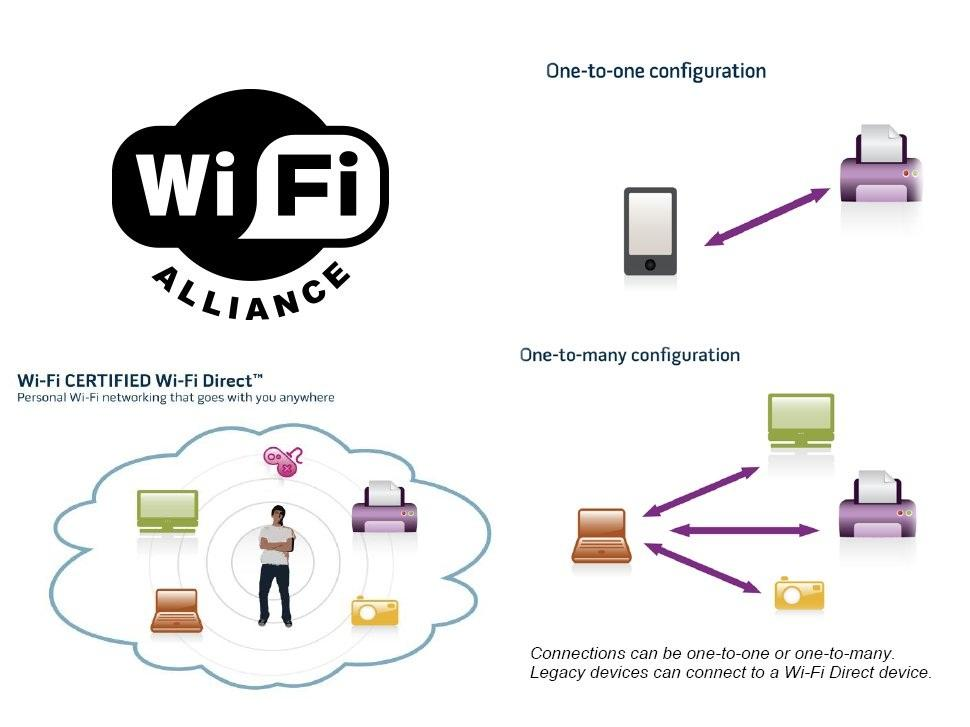
\includegraphics[width=1\textwidth]{imgs/wifi_alliance.jpg}
\captionof{figure}{Possibili utilizzi della tecnologia}\label{wifi_alliance_img}%
\end{center}

Nella figura  \ref{wifi_alliance_img} vengono mostrati i possibili utilizzi di questa tecnologia.
Nella One-to-one configuration notiamo che la connessione avviene tra uno smartphone e una stampante, in questo modo possiamo avere accesso alla stampante per stampare i file di relativo interesse.
Nella One-to-many configuration invece notiamo come la connessione avvenga tra più dispositivi ( in questa configurazione il Laptop sarà Il P2P GO e tutti gli altri i Client ), in questo modo si può interagire col P2P GO per avere accesso agli altri dispositivi, per esempio, dalla fotocamera inviare un file al PC oppure stampare direttamente una foto.
Oppure tramite lo stesso P2P GO si può avere accesso ai file degli altri dispositivi e stamparli inviandoli alla stampante.

\subsection{Formazione del P2P Group Owner}

Come detto in precedenza, perché la comunicazione tra due dispositivi avvenga c’è bisogno che venga instaurato un Group Owner ( GO ).
Wi-Fi Direct permette di creare tre gruppi differenti:

\subsubsection{Gruppo Standard}

In tale caso è necessario che i due dispositivi si trovino tramite la fase di Discover, e successivamente partirà la fase di negoziazione del GO.

\begin{center}
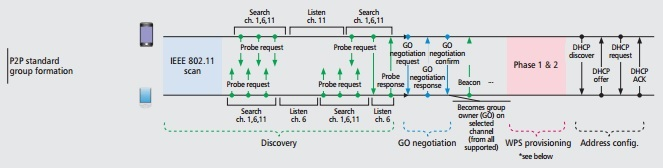
\includegraphics[width=1\textwidth]{imgs/Standard_Group.jpg}
\captionof{figure}{Illustrazione della formazione di un gruppo standard}\label{standard_group_img}%
\end{center}

Come si nota nella Figura \ref{standard_group_img} per prima cosa i P2P Devices selezionano uno dei tre canali ( 1, 6, 11 ) chiamati canali di ascolto.
Successivamente si alterneranno tra due stati: search e listen.
Nello stato di search i P2P Devices inviano un segnale ( di indagine ) chiamato Probe Request nei 3 canali.
Nello stato di listen invece, i P2P Devices saranno in ascolto sul proprio canale, in attesa di questo segnale ( Probe Request ) e saranno pronti a rispondere con il Probe Response.
Una volta che poi i due P2P Devices si sono trovati, inizierà la fase di negoziazione ( GO Negotiation ).
Per stabilire quindi chi sarà il GO e chi il Client, i due P2P Devices si invieranno un valore numerico ( GO Intent value ) tramite il meccanismo three-way handshake (  GO Negotiation Request/Response/Confirm ), e chi dichiarerà il valore più alto diventerà il P2P GO.
Per evitare qualsiasi tipo di conflitto in caso i due P2P Devices dichiarino lo stesso valore, è stato implementato un bit aggiuntivo ( tie-breaker).
Una volta che sono stati stabiliti i ruoli per i due P2P Devices, si passa all’ultima fase, che consiste nello stabilire una connessione sicura usando il Wi-Fi Protected Setup ( WPS Provisioning phase Figura 1.3 ) ed infine il settaggio di un indirizzo IP tramite lo scambio di DHCP.

\subsubsection{Gruppo Autonomous}

\begin{center}
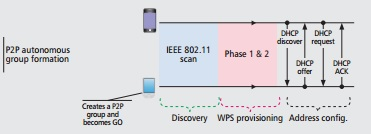
\includegraphics[width=1\textwidth]{imgs/Autonomous_Group.jpg}
\captionof{figure}{Illustrazione della formazione di un gruppo autonomo}\label{autonomous_group_img}%
\end{center}

Come si può notare dalla figura \ref{autonomous_group_img}, un P2P Device può creare autonomamente un P2P Group che diventa immediatamente il P2P GO, istanziandosi su un canale e cominciando a inviare segnali ( beacon ).
Gli altri dispositivi possono trovare tale gruppo con metodi tradizionali di scansione e procedere direttamente alla creazione della WPS Provisioning e all’Address Configuration.

\subsubsection{Gruppo Persistent}

\begin{center}
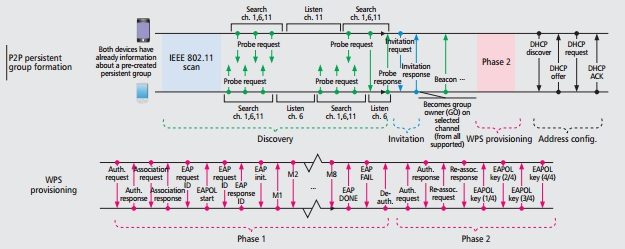
\includegraphics[width=1\textwidth]{imgs/Persistent_Group.jpg}
\captionof{figure}{Illustrazione della formazione di un gruppo persistente}\label{persistent_group_img}%
\end{center}

Come si può notare in figura \ref{persistent_group_img}, un P2P Device può essere in grado di riconoscere un gruppo già formato in precedenza usando i flag del P2P Capabilities presente nel Beacon frame, del Probe Response e del GO Negotiation.
In questo modo, se dopo la fase di Discovery un P2P Device riconosce che tale gruppo era già stato formato in precedenza con lo stesso peer.
Uno dei due P2P Device è in grado di ricreare quel gruppo tramite un processo di invito ( Invitation Procedure ) in modo molto veloce.

\subsection{Sicurezza ( WPS Provisioning )}

Come detto in precedenza, dopo che la fase di Discover è terminata e dopo che la negoziazione è finita, decidendo quindi chi ha il ruolo di P2P Group Owner e chi di Client, parte un ultima ma non meno importante fase, quella del WPS Provisioning.
I dispositivi che implementano Wi-Fi Direct devono implementare anche questo protocollo di sicurezza, in quanto si occupa di creare una connessione sicura tra i due, richiedendo il minimo sforzo all’utente.
Nello specifico, questo protocollo permette di creare una connessione sicura, richiedendo di immettere un determinato codice PIN dalla parte Client, oppure di premere un pulsante in tutti e due i dispositivi.
Per seguire le direttive del WPS, il P2P GO deve implementare il Registrar e il Client l’Enrollee.

\begin{center}
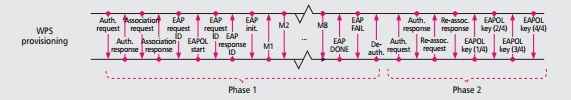
\includegraphics[width=1\textwidth]{imgs/WPS.jpg}
\captionof{figure}{Illustrazione del funzionamento del sistema di sicurezza WPS}\label{wps_img}%
\end{center}

Come possiamo vedere dalla Figura \ref{wps_img}, il WPS è composto da 2 fasi.
Nella prima fase il Registrar è incaricato di generare le credenziali per la connessione (  per esempio: chiave di sicurezza ) e di mandarle all’Enrollee.
Tali chiavi vengono generate col protocollo di sicurezza WPA-2, successivamente criptate tramite un protocollo chiamato AES-CCMP.
Nella seconda fase l’Enrollee ( Client ), si disconnette e si riconnette con le nuove credenziali inviategli dal Register.
Nel caso in cui alla riconnessione tutti e due i dispositivi abbiamo già le credenziali richieste si può procedere all’autenticazione, altrimenti si ripartirebbe dalla fase 1.



\section{Confronto con altre tecnologie}

Fino ad ora abbiamo spiegato nel dettaglio come funziona l’architettura WiFi Direct e abbiamo detto che si occupa di far comunicare due dispositivi senza bisogno di un hotspot, potremo dire quindi che è identico alla tecnologia Bluetooth, invece no, perché ha una grande differenza rispetto a quest’ultima, e cioè una migliore velocità nel trasferire le cose, tutto questo perché Wi-Fi Direct implementa per il trasferimento lo stesso protocollo di Wi-Fi.
Qui di seguito viene riportata una tabella che confronta tale tecnologia con Bluetooth:

\begin{center}
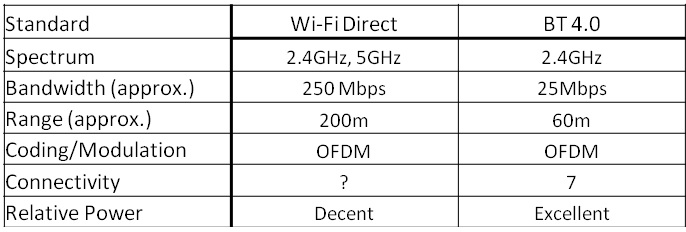
\includegraphics[width=1\textwidth]{imgs/WvsB.jpg}
\captionof{figure}{Wi-Fi Direct e Bluetooth messi a confronto}\label{WvsB_img}%
\end{center}

Per questo le varie applicazioni di questa tecnologia vanno pian piano ad espandersi, fino ad ora lo troviamo impiegato in: 
condivisione di file, sincronizzazione, stampa, video games e tutto ciò senza la necessità di trovare una connessione a internet per comunicare con i device.
Per la parte di applicazione lato condivisione di file lo troviamo nell’applicazione “Wi-Fi Shoot” che è un applicazione molto semplice, che permette una volta che i dispositivi si sono associati di scambiarsi file.
O ancora nell’applicazione “S-Beam” che permette sempre lo scambio di file effettuando un movimento ondulatorio verso l’altro dispositivo.
In ambito videogames invece, viene impiegato dal gioco “Spaceteam” un gioco di squadra in cui bisogna comunicare e dare direttive all’altra persona su cosa deve fare, in questo modo favorisce anche la socializzazione e la sincronizzazione, sia tra persone che tra dispositivi.


\clearpage{\pagestyle{empty}\cleardoublepage}
\chapter{Android & Wi-Fi direct}

Android è un sistema operativo per dispositivi mobili sviluppato da Google, basato su kernel Linux.
La sua progettazione è principalmente per smartphone e tablet, ma possiede anche interfacce utente specializzate per televisori (Android TV), automobili (Android  Auto), orologi da polso (Android Wear), occhiali (Google Glass) ecc… .
Essendo basato su kernel Linux possiede una licenza (Licenza Apache) che consente di modificare e distribuire liberamente il codice sorgente. 
Inoltre, tutte le applicazioni sono scritte soprattutto in linguaggio di programmazione Java.
Ogni release del sistema possiede un nome simbolico ed è rigorosamente dato seguendo l'ordine alfabetico, ed inoltre ogni nome corrisponde ad una golosità presente nel mondo, qua di seguito la lista delle varie versioni: la 1.5 venne chiamata Cupcake, la 1.6 Donut, la 2.1 Eclair, la 2.2 Froyo, la 2.3 Gingerbread, la 3.0 Honeycomb, la 4.0 Ice Cream Sandwich, la 4.1 Jelly Bean, la 4.4 Kit Kat. 
Attualmente l’ultima versione del sistema operativo è la 5.0, chiamata Lollipop.


\section{API}

\subsection{Architettura Android}

L'architettura di Android si suddivide in vari livelli (o layer), ognuno dei quali offre un servizio a quello superiore.
Vediamoli nel dettaglio:

\begin{center}
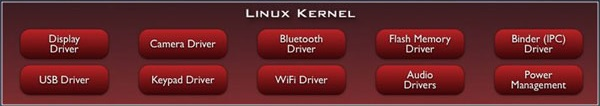
\includegraphics[width=1\textwidth]{imgs/Linux Kernel.jpg}
\captionof{figure}{Livello più basso dell'architettura Android}\label{linux_kernel_img}%
\end{center}

Nella figura \ref{linux_kernel_img} viene rappresentato il livello più basso di tale architettura, che contiene il kernel di Linux.
Inoltre, comprende anche vari driver per la gestione delle diverse periferiche: dallo schermo alla tastiera, dalla scheda di rete Wi-Fi all'alimentazione.

\begin{center}
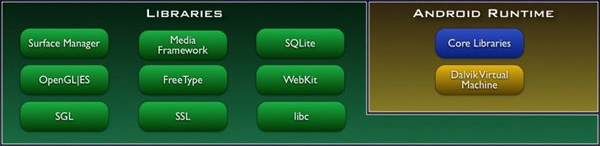
\includegraphics[width=1\textwidth]{imgs/Librerie.jpg}
\captionof{figure}{Tale livello rappresenta il cuore di Android}\label{librerie_img}%
\end{center}

Salendo invece al terzo livello, troviamo tutte le Librerie native che sono state svillupate nel linguaggio C/C++ figura \ref{librerie_img}.
Tutte insieme tali librerie rappresentano il cuore di Android, qui di seguito alcuni componenti delle librerie nello specifico: Surface Manager, che gestisce la componente grafica
Media Framework, implicata nella gestione dei codec audio e video
La libreria SSL che gestisce il Secure Socket Layer.

\begin{center}
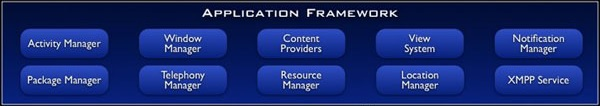
\includegraphics[width=1\textwidth]{imgs/Applicazioni_Framework.jpg}
\captionof{figure}{Livello composto da una serie di componenti API}\label{applicazioni_framework_img}%
\end{center}

Salendo ancora al quarto livello troviamo l'Application Framework figura \ref{applicazioni_framework_img}, formato da un insieme di API che svolgono specifici compiti:
Activity Manager, fondamentale in quanto è responsabile dell'interazione tra applicazione e utente.
Window Manager per la gestione delle finestre delle varie applicazioni.
Package Manager responsabile della gestione del ciclo di vita delle applicazioni.

\begin{center}
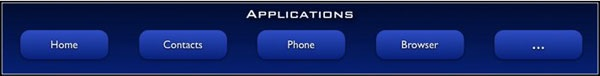
\includegraphics[width=1\textwidth]{imgs/Applicazioni.jpg}
\captionof{figure}{Ultimo livello che racchiude le applicazioni vere e proprie}\label{applicazioni_img}%
\end{center}

Arrivati all'ultimo livello, troviamo le Applicazioni vere e proprie che utilizzano i livelli sottostanti per essere eseguite figura \ref{applicazioni_img}.
Tra le tante applicazioni possiamo citare, calendario, rubrica, orologio.

\subsection{Ciclo di vita di un Applicazione (Activity)}

Nella sezione precedente abbiamo concluso parlando dell'ultimo livello, cioè quello che comprende le Applicazioni vere e proprie, un applicazione
è un software che viene eseguito e gestito dal sistema operativo Android, che possiede un proprio ciclo di vita.


\begin{center}
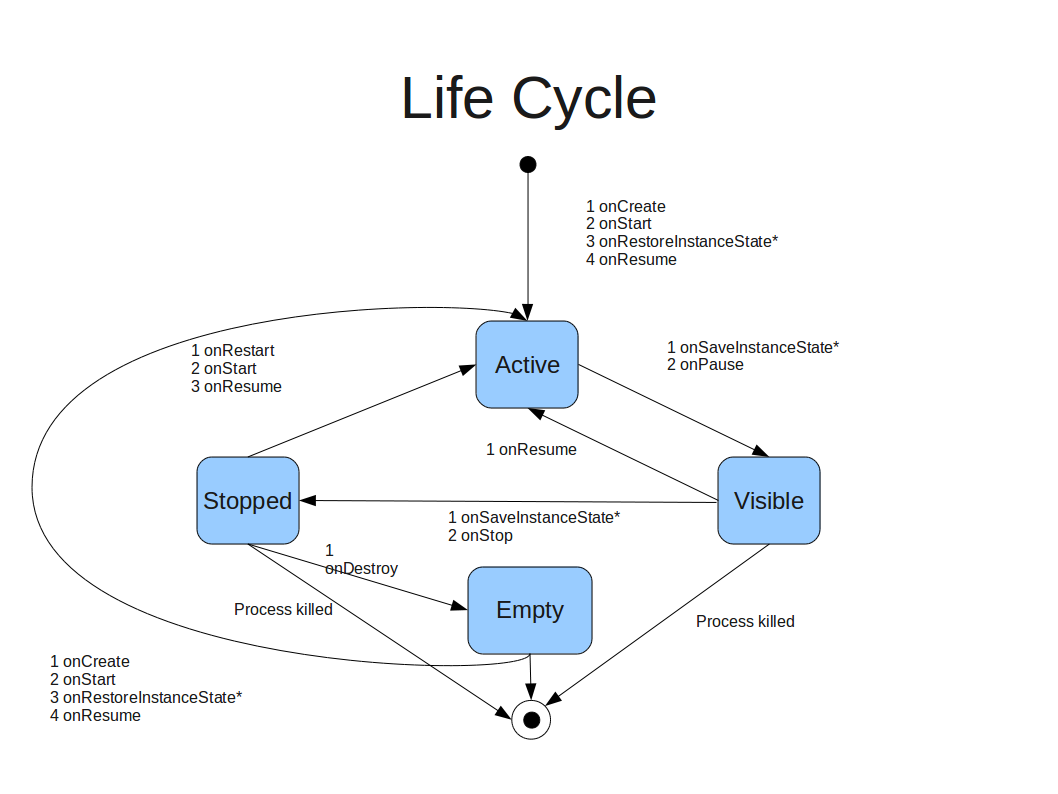
\includegraphics[width=1\textwidth]{imgs/ActivityLifeCycle.jpg}
\captionof{figure}{Rappresentazione ciclo di vita di un Activity}\label{activity_cycle_img}%
\end{center}

Come possiamo notare nella figura \ref{activity_cycle_img}, un ciclo di vita non è altro che una serie di stati attraverso i quali l'Activity passa.
I passaggi tra i diversi stati vengono notificati tramite una callback (metodo) invocata dal sistema.

Quando un activity viene mandata in esecuzione, vengono necessariamente invocati 3 metodi:
onCreate(): l'activity viene creata, e il programmatore dovrà definire le configurazione di base e il layout.

onStart(): l'activity diventa visibile, ed è il momento in cui i servizi e le funzionalità vengono attivate per fornire informazioni all'utente.

onResume(): l'activity diventa la destinazione di tutti gli input dell'utente.

Nel caso in cui l'Utente riceva una chiamata o più semplicemente apra un applicazione diversa, il sistema Android mette a risposo l'applicazione che stava usando in quel momento.
E anche per questa operazione verranno invocati 3 metodi:

onPause(): avverte che l'utente ha smesso di interagire con l'activity.

onStop(): indica la fine della visibilità dell'Activity.

onDestroy(): indica che l'Activity è stata terminata.

\section{Sketch codice}

\subsection{Wi-Fi Direct in Android}

Il Wi-Fi Direct chiamato anche Wi-Fi Peer to Peer (P2P) è disponibile sui dispositivi Android che posseggono la versione 4.0 (API 14), nonchè l'adeguato hardware.
Con tale tecnologia è possibile collegarsi e comunicare via Wi-Fi con un altro dispositivo, senza bisogno di un Access Point (AP) intermediario.

Tale tecnologia è basata su 2 parti fondamentali:

-Metodi, con la quale è possibile compiere le fasi di discover,request e connect verso i peer che sono indicati nella classe WifiP2PManager.

-Listener (oggetti), che si occupano di notificare il Successo o il Fallimento delle chiamate dei metodi contenuti nella classe WifiP2pManager.

-Intenti, che si occupano di notificare eventi specifici rilevati dal Wi-Fi P2P framework, per esempio una perdita di connessione o la scoperta di un nuovo peer.

Nella programmazione questi 3 metodi vengono usati spesso.
Un esempio pratico è l'uso di "WifiP2pManager.ActionListener" per chiamare il metodo discoverPeers(), se il metodo verrà eseguito correttamente verremo notificati dai metodi ActionListener.onSuccess() e ActionListener.onFailure().
Inoltre sarà anche trasmesso un intento chiamato WIFI P2P PEERS CHANGED ACTION nel caso in cui il metodo discoverPeers() rilevi modifiche tra la lista dei peer disponibili.

Per entrare ancora più nel dettaglio ecco una lista dei metodi, listener e intent contenuti nella classe WifiP2pManager:

\begin{center}
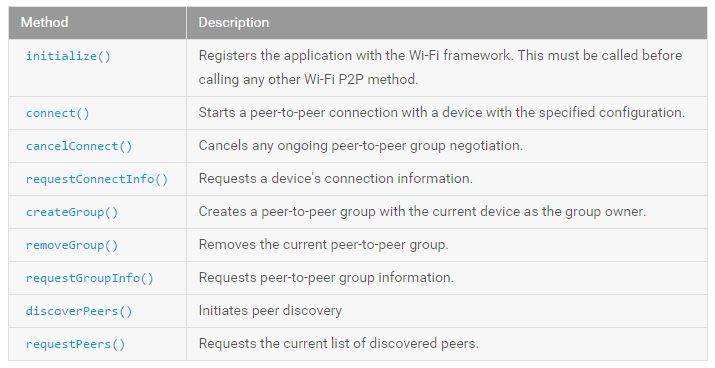
\includegraphics[width=1\textwidth]{imgs/p2pmethods.jpg}
\captionof{figure}{Lista dei Metodi persenti nella classe WifiP2pManager}\label{p2pmethods_img}%
\end{center}

\begin{center}
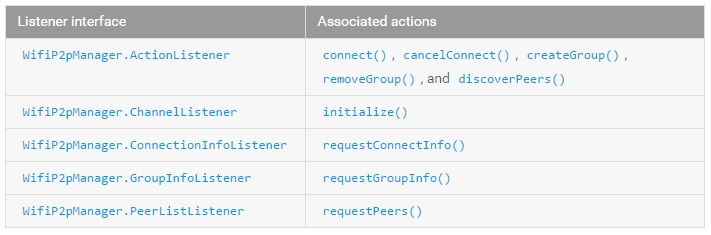
\includegraphics[width=1\textwidth]{imgs/p2plistener.jpg}
\captionof{figure}{Lista dei Listener persenti nella classe WifiP2pManager}\label{p2plistener_img}%
\end{center}

\begin{center}
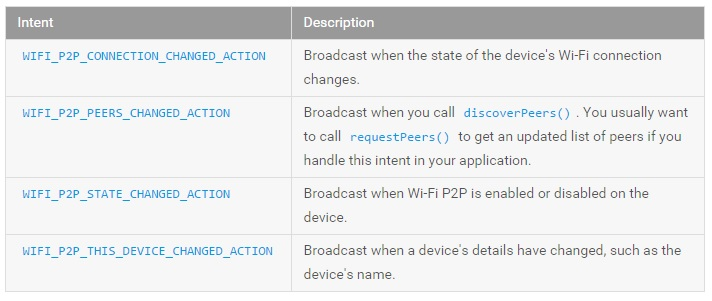
\includegraphics[width=1\textwidth]{imgs/p2pintents.jpg}
\captionof{figure}{Lista dei Intents persenti nella classe WifiP2pManager}\label{p2pintents_img}%
\end{center}

\subsection{Wi-Fi Direct in Pratica}

\subsubsection{Creazione classe BroadcastReceiver}

La creazione di una classe BroadcastReceiver è la base per lo sviluppo di un applicazione che vuole sfruttare il Wi-Fi Direct, in quanto permette di rispondere ad eventi (Intents) ricevuti di nostro interesse.
Ci sono 2 step base da seguire per la creazione di questa classe che permette di captare gli Intent Wi-Fi P2P e sono i seguenti:

1- Creazione di una classe che estenda la BroadcastReceiver.

2- Nella classe BroadcastReceiver eseguire la verifica degli Intent di nostro interesse all'interno del metodo       onReceive().
   Per esempio, se il BroadcastReceiver riceve un intento WIFI P2P PEERS CHANGED ACTION, si potrà chiamare il        metodo requestPeers() per avere una lista dei Peer trovati al momento.

   

\begin{center}
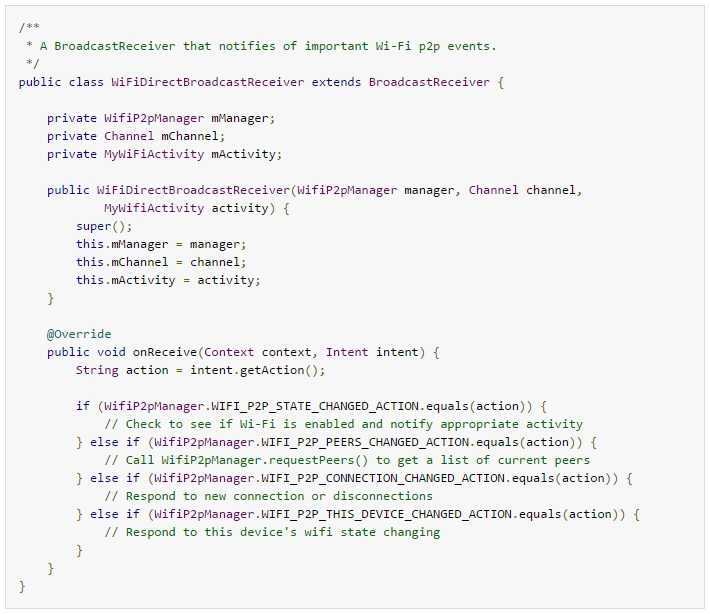
\includegraphics[width=0.9\textwidth]{imgs/broadcastreceiver.jpg}
\captionof{figure}{Rappresentazione classe BroadcastReceiver}\label{broadcastreceiver_img}%
\end{center}

\subsubsection{Creazione Applicazione Wi-Fi P2P}

Una volta creata la classe BroadcastReceiver possiamo procedere con lo sviluppo dell'applicazione vera e propria, di seguito seguiranno gli step passo passo.

1- Per prima cosa dobbiamo richiedere i permessi per usare l'hardware relativo al Wi-Fi, e per fare questo basta inserire il seguente codice all'interno di AndroidManifest:


\begin{center}
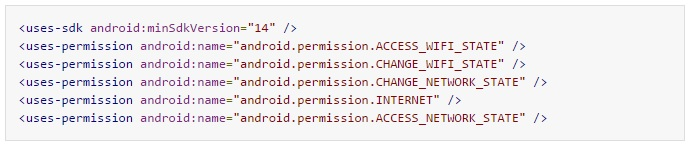
\includegraphics[width=1\textwidth]{imgs/manifest.jpg}
\captionof{figure}{Richiesta permessi di accesso a hardware Wi-Fi}\label{manifest_img}%
\end{center}

2- Eseguire un controllo sullo stato del Wi-Fi P2P ( acceso/spento, supportato o non supportato ): 
   
\begin{center}
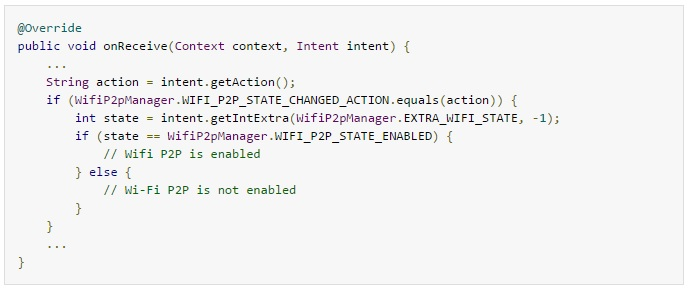
\includegraphics[width=1\textwidth]{imgs/check_wifi_avaiable.jpg}
\captionof{figure}{Controllo dello stato e del supporto del Wi-Fi P2P}\label{check_wifi_avaiable_img}%
\end{center}

3- All'interno del metodo onCreate(), bisogna creare un istanza WifiP2pManager e registrare la propria applicazione contenente il Wi-Fi P2P framework mediante il metodo initialize().
Tale metodo ritorna un WifiP2pManager.Channel (oggetto), con il quale sarà possibile connettersi al Wi-Fi P2P framework:

\begin{center}
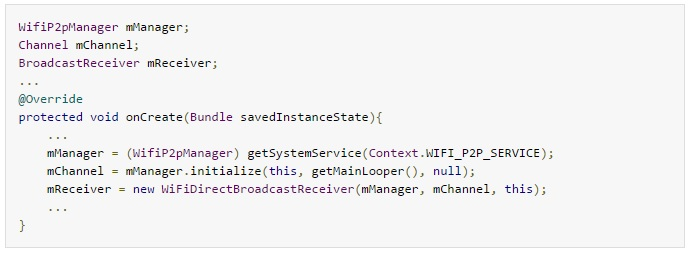
\includegraphics[width=1\textwidth]{imgs/onCreate.jpg}
\captionof{figure}{Metodo di connessione al framework}\label{onCreate_img}%
\end{center}

4- Creare un filtro di intenti, e aggiungere all'interno gli stessi intent contenuti nel BroadcastReceiver:

\begin{center}
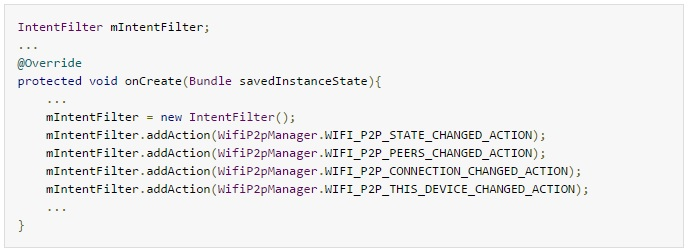
\includegraphics[width=1\textwidth]{imgs/intent_filter.jpg}
\captionof{figure}{Dichiarazione dei filtri per Intent}\label{intent_filter_img}%
\end{center}

5- Registrare il nostro BroadcastReceiver all'interno del metodo onResume() della nostra activity e cancellarlo dal metodo onPause():

\begin{center}
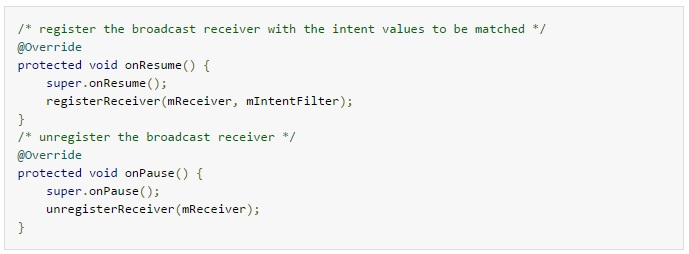
\includegraphics[width=1\textwidth]{imgs/register_receiver.jpg}
\captionof{figure}{Registrazione e cancellazione del BroadcastReceiver dai due metodi}\label{register_receiver_img}%
\end{center}

Una volta completati questi step, la tua applicazione sarà pronta per ricevere Wi-Fi P2P Intents ed effettuare chiamate dei metodi Wi-Fi P2P.

\subsubsection{Ricerca dei Peers (Utenti)}

Per ricevere la lista dei Peers disponibili alla connessione, bisogna effettuare una chiamata al metodo discoverPeers().
La chiamata di questo metodo funziona in modo asincrono, e il successo o fallimento di tale chiamata viene notificato dai metodi onSuccess() e onFailure() se è stato precedentemente creato un WifiP2pManager.ActionListener, da notare bene che tali metodi forniscono solo informazioni di successo o fallimento e non forniscono la lista dei peers appena trovati:

\begin{center}
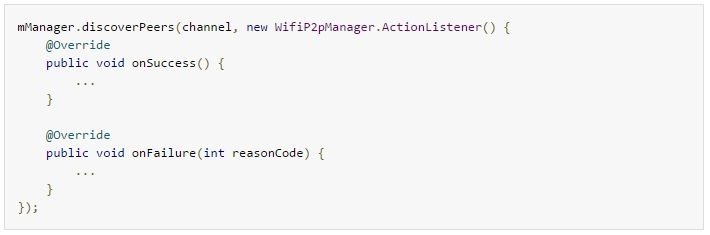
\includegraphics[width=1\textwidth]{imgs/discover_peers.jpg}
\captionof{figure}{Notifica di successo o fallimento per il metodo discoverPeers}\label{discover_peers_img}%
\end{center}

Se la fase di discoveri ha avuto successo e sono stati trovati nuovi Peers, il sistema di broadcast riceve un intento in WIFI P2P PEERS CHANGED ACTION, la lista dei peers si potrà ottenere tramite la chiamata del metodo requestPeers():

\begin{center}
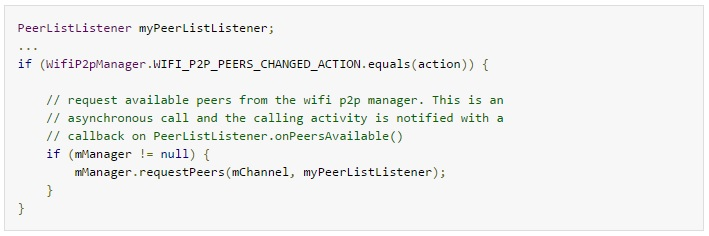
\includegraphics[width=1\textwidth]{imgs/intent_peers.jpg}
\captionof{figure}{Richiesta lista dei nuovi Peers}\label{intent_peers_img}%
\end{center}

Il metodo requestPeers() è anch'esso asincrono e può informare la nostra activity della presenza di una lista di nuovi Peers tramite il metodo onPeersAvailable() definito nell'interfaccia WifiP2pManager.PeerListListener.

\subsubsection{Connessione ai Peers}

Una volta trovato il dispositivo a cui vogliamo connetterci tra la lista dei Peers disponibili, sarà possibile connettersi ad esso tramite il metodo connect().
Tale metodo avrà bisogno di un oggetto WifiP2pConfig, all'interno del quale sono contenute le informazioni del dispositivo a cui vogliamo connetterci:

\begin{center}
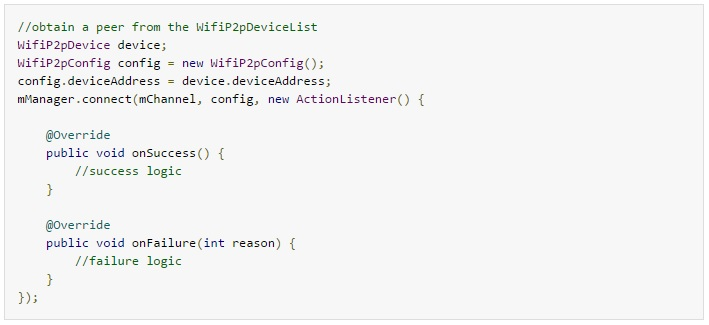
\includegraphics[width=1\textwidth]{imgs/connect.jpg}
\captionof{figure}{Metodo per permettere la connessione con un altro Peer}\label{connect_img}%
\end{center}

\subsubsection{Trasferimento Dati}

Una volta stabilita la connessione tra i due dispositivi, si può procedere con lo scambio di dati attraverso l'utilizzo di socket:

1- Creazione del ServerSocket, tale socket attenderà la connessione di un qualunque client sulla porta specificata e si bloccherà non appena l'avrà ricevuta (eseguire quindi questo processo all'interno di un thread).

2- Creazione di un ClientSocket, che userà indirizzo IP e porta definiti dal ServerSocket per connettersi ad esso.

3- Una volta che client e server saranno connessi si potrà procedere con lo scambio di dati tramite byte streams.

La figura \ref{server_img} illustrerà il codice impiegato lato Server per il trasferimento dei dati:


\begin{center}
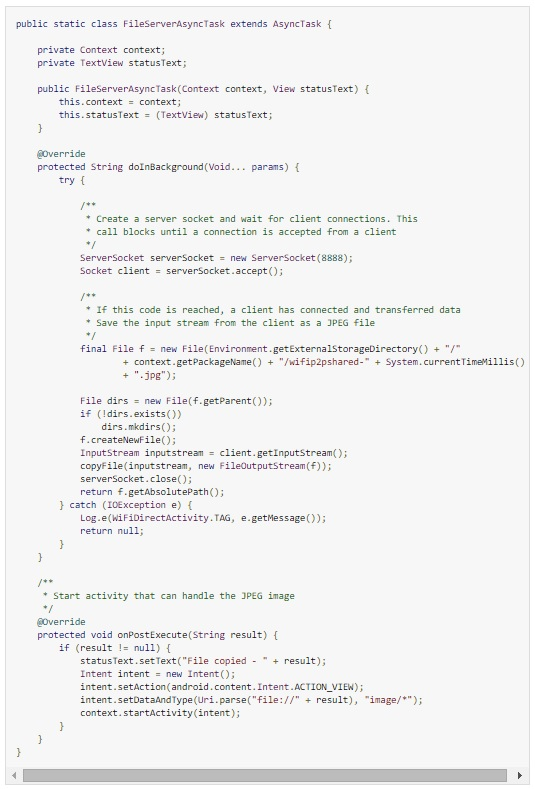
\includegraphics[width=1\textwidth]{imgs/server.jpg}
\captionof{figure}{Codice trasferimento dati lato Server}\label{server_img}%
\end{center}

La figura \ref{client_img} invece illustrerà la medesima cosa lato Client:

\begin{center}
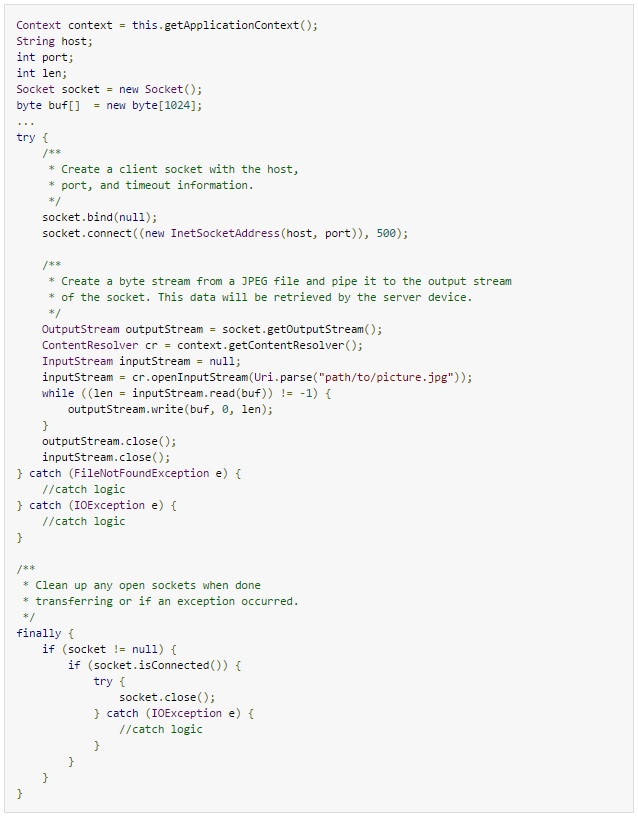
\includegraphics[width=1\textwidth]{imgs/client.jpg}
\captionof{figure}{Codice trasferimento dati lato Server}\label{client_img}%
\end{center}

\clearpage{\pagestyle{empty}\cleardoublepage}
\part{Parte sperimentale}
\chapter{Valutazione sperimentale delle prestazioni}
In questo capitolo analizzeremo nel dettaglio l'applicazione da me realizzata per lo svolgimento dei test su tale tecnologia.

\section{Applicazione}
Per la realizzazione di tali test sono stati impiegati 2 dispositivi.
Il primo dispositivo avrà la funzione di P2P Group Owner (Server), mentre invece il secondo avrà la funzione di Client.

\subsection{P2P Group Owner}
I test sono stati eseguiti con l'ausilio di un gruppo standard:
L'utilizzo di tale gruppo, come spiegato precedentemente, implica che prima che venga deciso quale dei due dispositivi sarà il Group Owner (GO), bisognerà attraversare un fase chiamata di negoziazione (GO Negotiation), in tale fase i due dispositivi decideranno su quale canale (1,6,11) porsi, ed inizieranno ad inviarsi valori numerici tra loro che dichiareranno in seguito.
Alla fine chi avrà dichiarato il valore più alto assumerà il ruolo di Grou Owner ed inizieranno a comunicare.

La comunicazione lato server avviene tramite la creazione di un Thread chiamato ThreadCalcoli (in cui verranno effettuati i calcoli delle due metriche: Packet Delivery Ratio e Throughput) che a sua volta creerà un secondo Thread chiamato ThreadComunicazione (che si occuperà esclusivamente di ricevere e reinviare i pacchetti ottenuti dal Client).
Una volta creato il ThreadComunicazione, il ThreadCalcoli andrà in stato di sleep per un totale di 50 secondi.
Tale Thread invece rimarrà in attesa dei pacchetti che verranno inviati dal Client.
Durante il processo, sono state istanziate 2 variabili che saranno fondamentali per il calcolo delle 2 metriche e che verranno condivise tra i 2 Thread.
La prima variabile sarà utile a ricavare il Throughput su 50 secondi, assumendo il valore della dimensione del pacchetto ricevuto, mentre invece la seconda avrà lo scopo di contatore per tenere traccia del numero di pacchetti ricevuti, utile per calcolare il Packet Delivery Ratio.
Una volta che il ThreadCalcoli ha raggiunto i 50 secondi, invia un segnale al ThreadComunicazione bloccandolo, permettendo così il calcolo delle 2 metriche attraverso la lettura dei dati ricevuti contenuti nelle 2 variabili.
Terminati tali calcoli il ThreadCalcoli sblocca il ThreadComunicazione e si rimette in stato di sleep per altri 50 secondi ripetendo successivamente le stesse operazioni per i cicli successivi.

\subsection{Client}
Tale dispositivo si occupa di inviare i pacchetti al Server, l'invio di tali pacchetti avviene attraverso la lettura di un array chiamato packets che contiene il numero di pacchetti da inviare.


\section{Dispositivi usati}
Per la realizzazione di tali esperimenti sono stati usati i seguenti dispositivi:

-Samsung Galaxy S5

\begin{center}
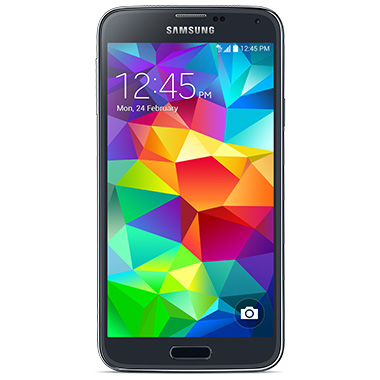
\includegraphics[width=1\textwidth]{imgs/s5.jpg}
\captionof{figure}{Samsung Galaxy S5}\label{s5_img}%
\end{center}

-Google Nexus 5

\begin{center}
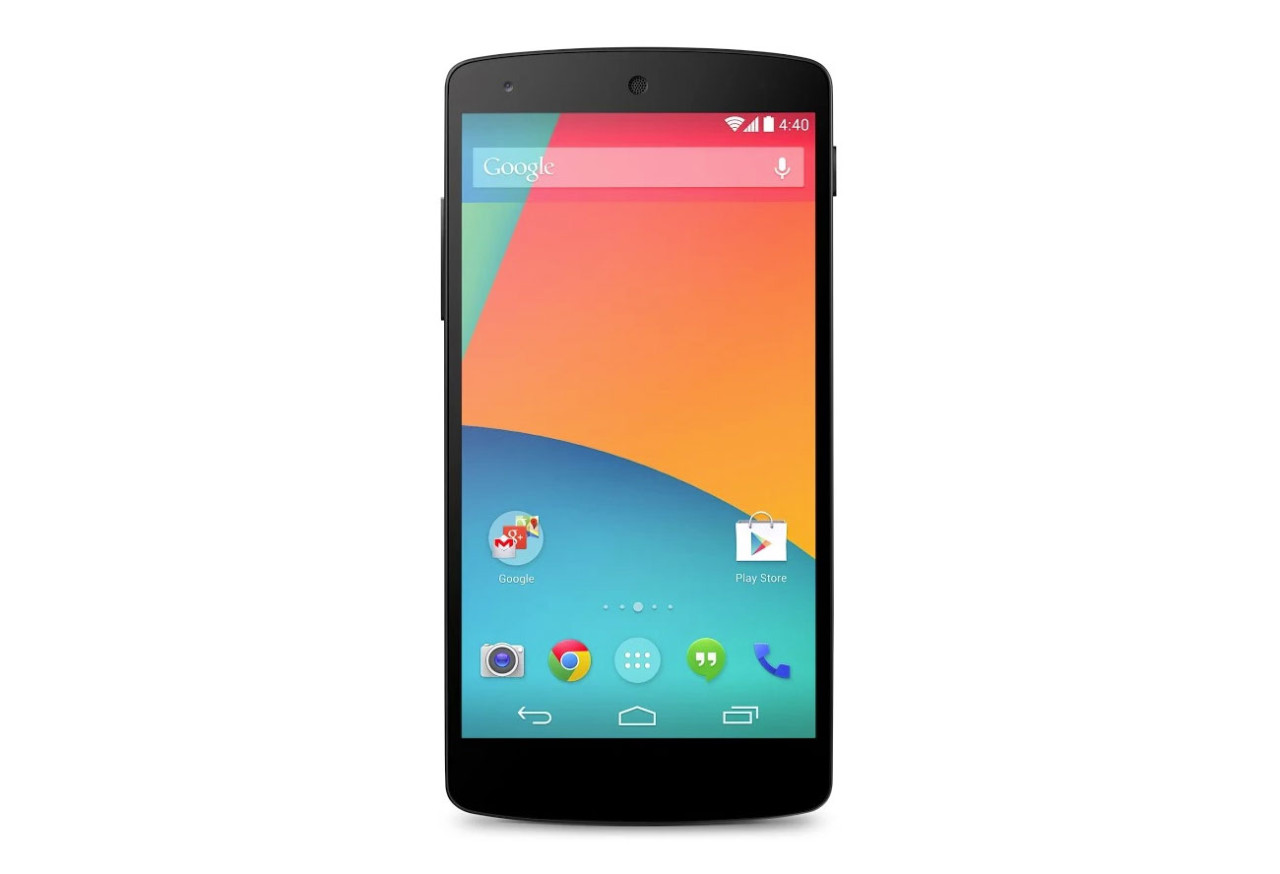
\includegraphics[width=1\textwidth]{imgs/nexus5.jpg}
\captionof{figure}{Google Nexus 5}\label{nexus_5_img}%
\end{center}

\section{Esperimenti}
Per effettuare il calcolo delle 3 metriche ho eseguito i test in 2 ambienti:Indoor e Outdoor.

\subsection{Packet Delivery Ratio (PDR)}





Per eseguire il calcolo di tale metrica ho impostato l'array packets con una serie di valori che indicano il numero di pacchetti da inviare figura \ref{}, variando la distanza dei dispositivi ogni volta che l'intera applicazione terminava il processo.

\subsection{Throughput}





Per eseguire il calcolo di tale metrica ho impostato un tempo pari a 50 secondi e una dimensione del singolo pacchetto di 1000 Byte.
Il test quindi ha 9 cicli della durata di 50 secondi con un numero di pacchetti diverso ad ogni ciclo, inoltre al termine dell'intero processo la distanza tra i dispositivi viene variata.

\subsection{Discovery Time}




Per eseguire il calcolo di tale metrica ho usufruito di 2 tipologie di gruppi per la decisione del Group Owner: Gruppo standard e Gruppo Autonomo.
Nel caso del gruppo standard l'associazione tra i due dispositivi avviene tramite una semplice discovery, che implicherà però il passaggio attraverso una fase di GO Negotiation per decidere chi sarà Group Owner.





Nel caso del gruppo autonomo invece, tale fase non viene eseguita, e quindi il dispositivo diventerà subito il Group Owner e gli altri potranno associarsi tramite una semplice discovery.
Nel calcolo di tale metrica è stato effettuato anche un ulteriore esperimento connettendo tra loro più dispositivi.


\section{Metriche}
Qui di seguito riporterò le formule utilizzate per il calcolo delle 3 metriche.

\subsection{Packet Delivery Ratio (PDR)}
\begin{center}

\includegraphics[width=1\textwidth]{imgs/PDR.jpg}
\captionof{figure}{Formula calcolo Packet Delivery Ratio}\label{PDR_img}%
\end{center}

Rapporto fra il numero di pacchetti ricevuti a destinazione e il numero di pacchetti inviati dalla sorgente.
Dove x rappresenta il numero di pacchetti inviati dalla sorgente e y il numero di quelli ricevuti a destinazione figura \ref{PDR_img}. 

\subsection{Throughput}
\begin{center}

\includegraphics[width=1\textwidth]{imgs/Throughput.jpg}
\captionof{figure}{Formula calcolo Throughput}\label{Throughput_img}%
\end{center}

Rappresenta l’effettiva quantità di byte trasmessi in una determinata quantità di tempo figura \ref{Throughput_img}.
Negli esperimenti è stato considerato un tempo di 50 secondi e una dimensione dei pacchetti di 1000 Byte.

\subsection{Discovery Time}

Il calcolo del Discovery Time indica il tempo impiegato dai 2 dispositivi per trovarsi e associarsi.





\clearpage{\pagestyle{empty}\cleardoublepage}
\chapter{Risultati}
In questo capitolo, ci si è occupati di eseguire i test delle metriche sul Wi-Fi Direct, in due tipologie ambientali: Indoor e Outdoor. 
Nei test eseguiti, è stato riscontrato che nel caso outdoor, i due smartphone hanno una portata di ricezione massima fino a 80 metri, mentre nei test indoor fino a 20 metri.
\newpage

\section{Analisi 1: Packet Delivery Ratio}

Ambiente Indoor:
\begin{center}
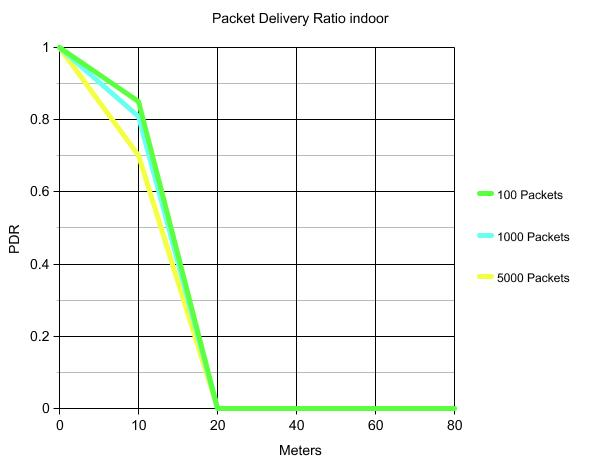
\includegraphics[width=1\textwidth]{imgs/PDR_Indoor_New.jpg}
\captionof{figure}{Rappresentazione in percentuale invio e ricezione pacchetti ambiente Indoor}\label{pdr_indoor_img}%
\end{center}

Come possiamo notare dalla figura \ref{pdr_indoor_img}, nell'asse delle ordinate sono stati posti i valori del range di distanza tra i due dispositivi misurati in metri, mentre nelle ordinate la percentuale di pacchetti che viene trasmessa e ricevuta.
Abbiamo analizzato 3 campioni composti rispettivamente da: 100, 1000 e 5000 pacchetti.
Si noti come all'aumentare della distanza la percentuale dei pacchetti trasmessi e ricevuti cali drasticamente fino ad arrivare a 0 raggiunti i 20 metri, ciò è causato anche dalla presenza di ostacoli ( muri ) avendo compiuto l'esperimento all'interno di una struttura.

Ambiente Outdoor:
\begin{center}
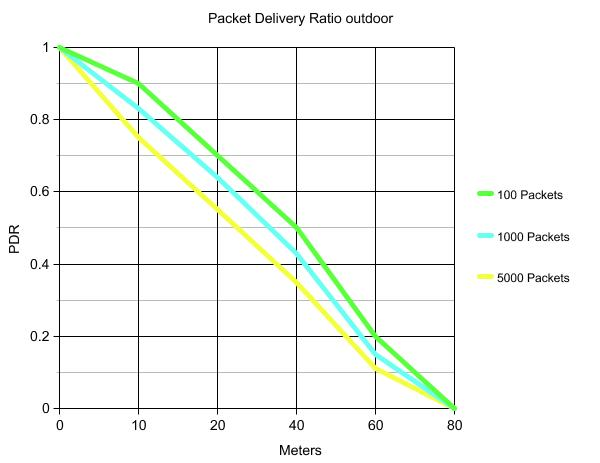
\includegraphics[width=1\textwidth]{imgs/PDR_Outdoor_New.jpg}
\captionof{figure}{Rappresentazione in percentuale invio e ricezione pacchetti ambiente Outdoor}\label{pdr_outdoor_img}%
\end{center}

Nel caso dell'ambiente outdoor, possiamo notare in figura \ref{pdr_outdoor_img} come invece la situazione tenda a migliorare, riuscendo a raggiungere una distanza di trasferimento e ricezione massima di 80 metri.
Nel caso outdoor è stata prestata molta attenzione nell'eseguire i test senza alcun tipo di ostacolo tra i due dispositivi.
\newpage

\section{Analisi 2: Throughput}

Ambiente Indoor:
\begin{center}
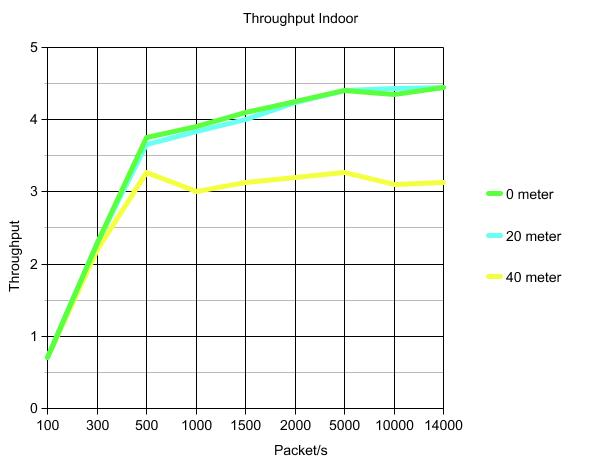
\includegraphics[width=1\textwidth]{imgs/ThroughputIndoor.jpg}
\captionof{figure}{Rappresentazione in Megabit (Mb) della quantità massima di dati inviabili in ambiente Indoor}\label{throughputindoor_img}%
\end{center}

Come possiamo notare nella figura \ref{throughputindoor_img}, nell'asse delle ordinate sono stati posti i valori che indicano il numero di pacchetti inviati da un dispositivo ad un altro fino ad un massimo di 14000, in quello delle ascisse invece la quantità di dati trasmessa in Megabit (Mb) fino ad un massimo di 5.
Ogni linea del grafico rappresenta una distanza diversa tra i dispositivi, rispettivamente: 0 metri, 10 metri e 20 metri.
Si noti come non si superino i 5Mb e nel caso dell'ultima linea di distanza (20 metri) come sia presente una perdita significativa di byte, mentre invece nel caso delle altre 2 come convergano nel medesimo punto.

Ambiente Outdoor:
\begin{center}
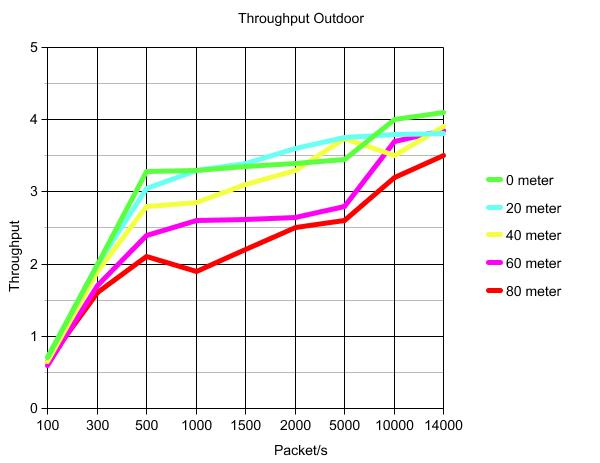
\includegraphics[width=1\textwidth]{imgs/ThroughputOutdoor.jpg}
\captionof{figure}{Rappresentazione in Megabit (Mb) della quantità massima di dati inviabili in ambiente Indoor}\label{throughputoutdoor_img}%
\end{center}

Come possiamo notare nella figura \ref{throughputoutdoor_img} anche nel caso outdoor non si superano i 5 Mb, ma si noti anche come le linee che rappresentano rispettivamente le distanze: 0, 20, 40, 60 e 80 metri convergano quasi negli stessi punti, fatta eccezione per gli 80 metri in cui si comincia ad intravedere una discreta perdita di Byte.

\section{Analisi 3: Discovery Time}
Come detto in precedenza, per tale metrica sono stati effettuati 2 tipi di test diversi con più dispositivi: 

-Discovery Time without Group Owner
-Discovery Time with Group Owner

\subsection{Discovery Time without Group Owner (GO)}

Ambiente Indoor:
\begin{center}
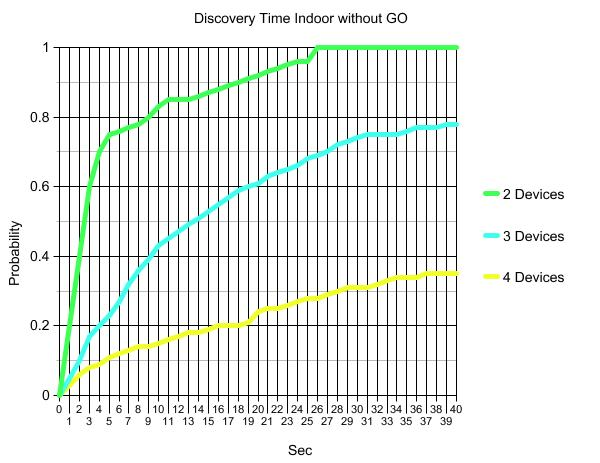
\includegraphics[width=1\textwidth]{imgs/Discovery_Time_Indoor_no_GO.jpg}
\captionof{figure}{Rappresentazione tempo associazione tra più dispositivi senza Group Owner in ambiente Indoor}\label{discoverytimeindoornogo_img}%
\end{center}

Nella figura \ref{discoverytimeindoornogo_img} è stato rappresentata in percentuale la probabilità di associazione tra più dispositivi, ponendo nelle asse delle ordinate i secondi impiegati e nelle asse delle ascisse la percentuale.
Da tale grafico si può notare come due dispositivi abbiamo probabilità molto alta di completare con successo l'associazione diventando certa dopo un tempo di 26 secondi.
Caso diverso invece per quanto riguarda l'associazione tra 3 e 4 dispositivi presentado una probabilità alquanto bassa, nel caso di 3 dispositivi dopo i 40 secondi siamo ancora su una probabilità di 0.8, mentre invece nel caso di 4 dispositivi siamo sullo 0.4.

Ambiente Outdoor:
\begin{center}
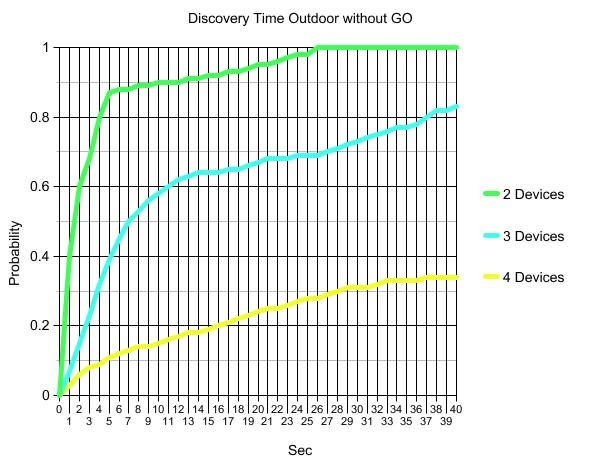
\includegraphics[width=1\textwidth]{imgs/Discovery_Time_Outdoor_no_GO.jpg}
\captionof{figure}{Rappresentazione tempo associazione tra più dispositivi senza Group Owner in ambiente Outdoor}\label{discoverytimeoutdoornogo_img}%
\end{center}

Nella figura \ref{discoverytimeoutdoornogo_img} si nota invece un discreto miglioramento per quanto riguarda l'associazione tra 2 e 3 dispositivi, mentre invece la situazione rimane tale per il caso dei 4 dispositivi.
\newpage

\subsection{Discovery Time with Group Owner (GO)}

Ambiente Indoor:
\begin{center}
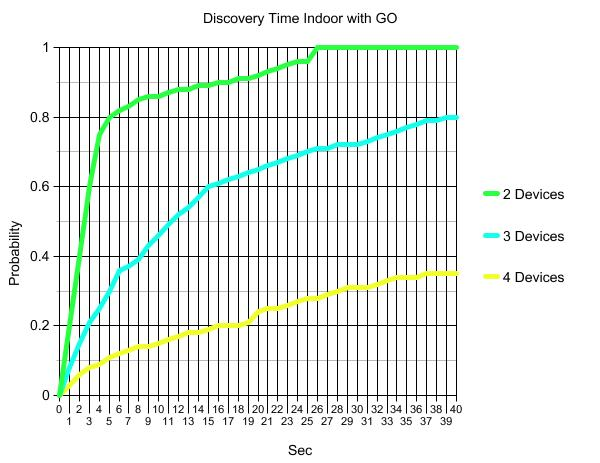
\includegraphics[width=1\textwidth]{imgs/Discovery_Time_Indoor_with_GO.jpg}
\captionof{figure}{Rappresentazione tempo associazione tra più dispositivi senza Group Owner in ambiente Outdoor}\label{discoverytimeindoorwithgo_img}%
\end{center}

Come possiamo notare dalla figura \ref{discoverytimeindoorwithgo_img}, possiamo notare miglioramenti rispetto al test di prima con una probabilità di successo di associazione di 0.8 a 5 secondi per 2 dispositivi, mentre invece di 0.6 a 15 secondi per 3 dispositivi, per il caso di 4 dispositivi invece si rimane sempre sullo 0.4.
\newpage

Ambiente Outdoor:
\begin{center}
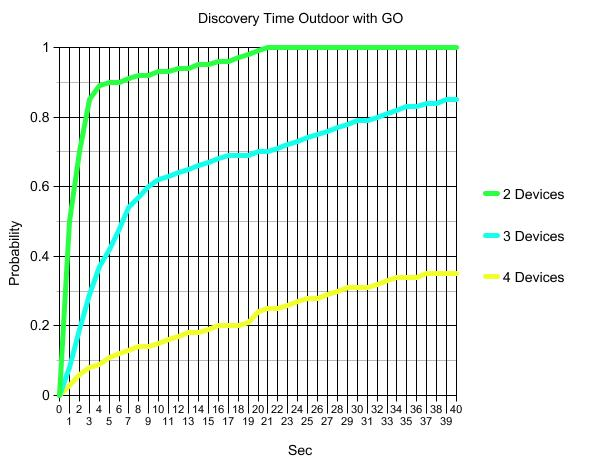
\includegraphics[width=1\textwidth]{imgs/Discovery_Time_Outdoor_with_GO.jpg}
\captionof{figure}{Rappresentazione tempo associazione tra più dispositivi senza Group Owner in ambiente Outdoor}\label{discoverytimeoutdoorwithgo_img}%
\end{center}

Dalla figura \ref{discoverytimeoutdoorwithgo_img}, possiamo notare che anche nel caso Outdoor si sono presentati notevoli miglioramenti, con una probabilità di successo di 0.9 a 5 secondi per il caso di 2 dispositivi, sempre una probabilità di successo dello 0.6 ma stavolta a 9 secondi, mentre invece per il caso di 4 dispositivi rimane sempre allo 0.4.
\newpage

Quindi, riassumendo tutti e 4 i grafici in uno solo:
\begin{center}
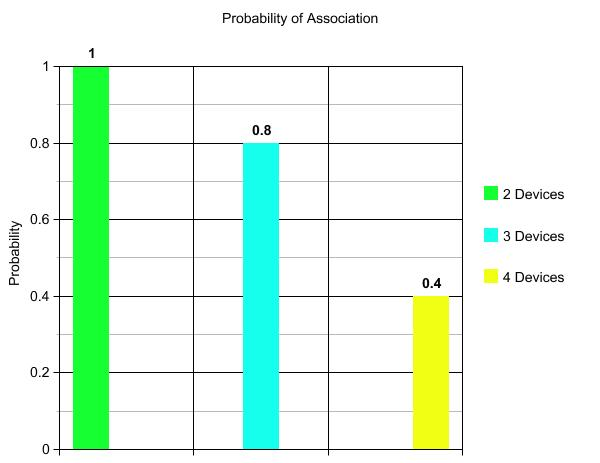
\includegraphics[width=1\textwidth]{imgs/probability_of_association.jpg}
\captionof{figure}{Rappresentazione tempo associazione tra più dispositivi senza Group Owner in ambiente Outdoor}\label{probabilityofassociation_img}%
\end{center}

In conclusione si può notare che la probabilità di associazione tra 2 dispositivi è pari ad 1 (quindi una certezza), mentre invece per il caso di 3 dispositivi o 4 dispositivi la probabilità massima è rispettivamente di 0.6 e 0.4.

\clearpage{\pagestyle{empty}\cleardoublepage}
\chapter{Conclusioni}
Nella tesi è stato inizialmente descritto lo standard Wi-Fi Direct, approfondendo successivamente anche il suo funzionamento e la sua architettura.
Dopodichè è stato descritto nel dettaglio il sistema operativo Android, e le applicazioni che tale tecnologia può avere su esso.
Dopo questa parte teorica, è stata trattata la fase sperimentale, in cui sono stati effettuati e descritti determinati test per la valutazione delle metriche.
Con esse ci si è potuti rendere conto delle reali potenzialità di tale tecnologia.
Parlando nel dettaglio, nel caso del Packet Delivery Ratio e del Throughput, ci si è resi conto che le prestazioni risultano basse in ambienti Indoor, in quanto essendo all'interno di strutture, sono presenti ostacoli tra i dispositivi (muri) che ne riducono l'efficenza.
Mentre invece nel caso Outdoor otteniamo risultati molto migliori, in quanto (grazie anche ad un attenzione molto curata) non è presente nessun tipo di ostacolo tra i 2 dispositivi.
Inoltre tali test sono stati ripetuti anche usando dispositivi meno recenti, e si è appurato che esiste una differenza in ambito di prestazioni, tra dispositivi "vecchi" (Samsung Galaxy S3 e Samsung Galaxy Tab 2) e dispositivi "nuovi" (Samsung Galaxy S5 e Google Nexus 5), un esempio pratico lo si può trovare nei grafici precedentemente descritti, dove si è arrivati ad avere una distanza massima tra i due dispositivi (in ambiente outdoor) pari a 80 metri, quando invece la distanza massima per dispositivi vecchi era 60-65 metri.
Un altra scoperta è stata nel calcolo del Discovery Time, dove si è appurato che i test dove veniva implementato il Group Owner risultavano migliori rispetto a quello senza GO, questo perchè con l'utilizzo del Group Owner si può saltare la fase di negoziazione (fase in cui i due dispositivi perdono tempo a decidere chi dovrà essere il server e chi il client).
Inoltre si è constatato anche che il numero massimo di dispositivi associabili tra loro è pari a 4, anche se in verità raramente la connessione tra tutti e 4 i dispositivi avviene, infatti dopo 40 secondi la probabilità che l'associazione sia terminata è pari a 0.4.

\section{Sviluppi Futuri}

Visto i risultati che sono stati ottenuti, si potrebbe pensare di approfondire alcuni concetti per l'impiego di tale tecnologia, come per esempio l'uso in ambito Videogames, per permettere partite fino a 4 Giocatori create in Locale.
Oppure cercare di ottimizzare tale tecnologia per un uso ottimale in mobilità.

\clearpage{\pagestyle{empty}\cleardoublepage}
\chapter{Bibliografia}

1- Device-to-Device Communications with Wi-Fi Direct: Overview and
   experimentation (Daniel Camps-Mur, Nec Network Laboratories, Andreas
   Garcia-Saavedra and Pablo Serrano, Universidad Carlos III De Madrid)
   
2- http://ieeexplore.ieee.org/xpl/login.jsp?tp=&arnumber=6549288&url=http%3A%    2F%2Fieeexplore.ieee.org%2Fstamp%2Fstamp.jsp%3Ftp%3D%26arnumber%3D6549288

3- http://www.html.it/pag/48652/il-ciclo-di-vita-di-unactivity/

4- http://developer.android.com/guide/topics/connectivity/wifip2p.html

5- Device-to-device communications with Wi-Fi Direct: overview and
   experimentation (Daniel Camps-Mur, Andres Garcia-Saavedra and Pablo Serrano)
   


\end{document}